\documentclass{article}
% \usepackage{xeCJK}
\usepackage{amsmath}
\usepackage{amssymb}
\usepackage{mathrsfs}
\usepackage{xcolor}
\usepackage{bm}
\usepackage{hyperref}
\usepackage{graphicx}
\usepackage{subcaption}
\usepackage{float}
\usepackage{multicol}
\usepackage{pdfpages}
\usepackage[ruled,linesnumbered]{algorithm2e}
\usepackage[numbers, sort&compress]{natbib}

\bibliographystyle{plain}
\setlength{\parindent}{2em}
\usepackage{geometry}
\geometry{a4paper, left=2.54cm, right=2.54cm, top=3.18cm, bottom=3.18cm}

% set line spacing
% \renewcommand{\baselinestretch}{1.5}

% define reference format
\hypersetup{
    colorlinks=true,
    linkcolor=blue,
    urlcolor=blue,
    citecolor=blue,
    linkbordercolor=white
}

\title{\textbf{Phase Frustration-Induced Crystallize in Chiral Active Matter}}
\author{Yichen Lu and Yiyi Zhang}

\begin{document}

\maketitle

\tableofcontents

% \newpage
\section{The Model}

Particles have a spatial position $\mathbf{r}_i=\left( x_i, y_i \right)$ and an internal phase $\theta_i$ which evolve according to equations:
\begin{subequations} 
    \label{eq:totalDynamicsMeanField}
    \begin{align}
        \dot{\mathbf{r}}_i&=v\mathbf{p}\left( \theta _i \right)\;\label{eq:dotR},
        \\
        \dot{\theta}_i&=\omega _i+\frac{K}{\left| A_i \right|}\sum_{j\in A_i}{\left[ \sin \left( \theta _j-\theta _i+\alpha \right) -\sin \alpha \right]}\;\label{eq:dotTheta},
    \end{align}
\end{subequations}
for $i=1,2,\ldots,N$. Here in Eq.~(\ref{eq:dotR}), $\mathbf{p}\left( \theta \right) =\left( \cos \theta ,\sin \theta \right)$, which means each particle rotates with a constant speed $v$ in the direction of its instantaneous phase $\theta_i (t)$. 
The particles are treated as point-like with no direct spatial interactions, consistent with classical models of chiral self-propelled particles \cite{PhysRevResearch.1.023026,PhysRevLett.119.058002,Fruchart2021,PhysRevLett.127.238001,PhysRevLett.133.258302}.
As per Eq.~(\ref{eq:dotTheta}), the mean runs over neighbors within a coupling radius $d_0$ around particle $i$:
\begin{equation}
    A_i\left( t \right) =\left\{ j\mid \left| \mathbf{r}_i\left( t \right) -\mathbf{r}_j\left( t \right) \right|\leqslant d_0 \right\} \;,
\end{equation}
$K$ is the coupling strength, and $\omega_i$ is the natural frequency of the $i$-th particle. 
This means that a particle will rotate with the angular velocity $|\omega_i |$ in the absence of mutual coupling ($K=0$), and the sign of $\omega_i$ represents the direction of rotation, namely, the tribute of the chirality of the $i$-th particle. A positive (negative) chirality ($\omega$) describes the counterclockwise (clockwise) rotations of the particle in space. 
We will study particles including two types of chiralities with both positive and negative natural frequencies uniformly distributed in two symmetric regimes as 
\begin{equation}
    g_U^{D}\left( \omega ;\mu,\sigma\right) 
    =\frac{1}{2}\left [
    g_U\left( \omega ;-\mu,\sigma\right) + 
    g_U\left( \omega ; \mu,\sigma\right) \right ].
    \label{eq:uniform2}
\end{equation}
where $g_U\left( \omega ;\mu ,\sigma \right)$ is the uniform distribution:
\begin{equation}
    g_U\left( \omega ;\mu ,\sigma \right) =\begin{cases}
	\frac{1}{\sigma},&		\omega _{\min}\leqslant \omega \leqslant \omega _{\max}\\
	0,&		\mathrm{otherwise}\\
\end{cases}\;.
\label{eq:uniform}
\end{equation}
Here $\sigma = \omega_{\max}-\omega _{\min}$ is the natural-frequency span, and $\mu = (\omega_{\max}+\omega _{\min})/2$ is the average.

Additionally, $\alpha$ is the phase frustration between two neighboring particles. When $\alpha_0=0$, the dynamics reduces to the normal chiral model \cite{LU2025115794}. 
The counter term $-\sin\alpha$ is introduced to ensure that frustration only interferes with the phase coupling without changing the sign of effective frequency. 

\section{Phase frustration-induced crystallization}
\subsection{Key properties}
\begin{enumerate}
    \item What does the lattice structure look like?
    \item What is each cell composed of?
    \item What is the unit cell structure, and what is the spatial arrangement of the unit cells?
    \item What is the internal dynamics within a cell?
    Besides triangular, what other spatial structures exist?
    \item What determines the length (periodicity)? (Interaction distance?)
    In which regions of frustration does it appear? (And what are the corresponding coupling conditions and natural frequency distributions?)
\end{enumerate}

\subsection{Mechanism}
What is the mechanism behind the formation of this phenomenon?

\section{Continuum model (Theoretical Analysis)}

\begin{figure}
    \centering
    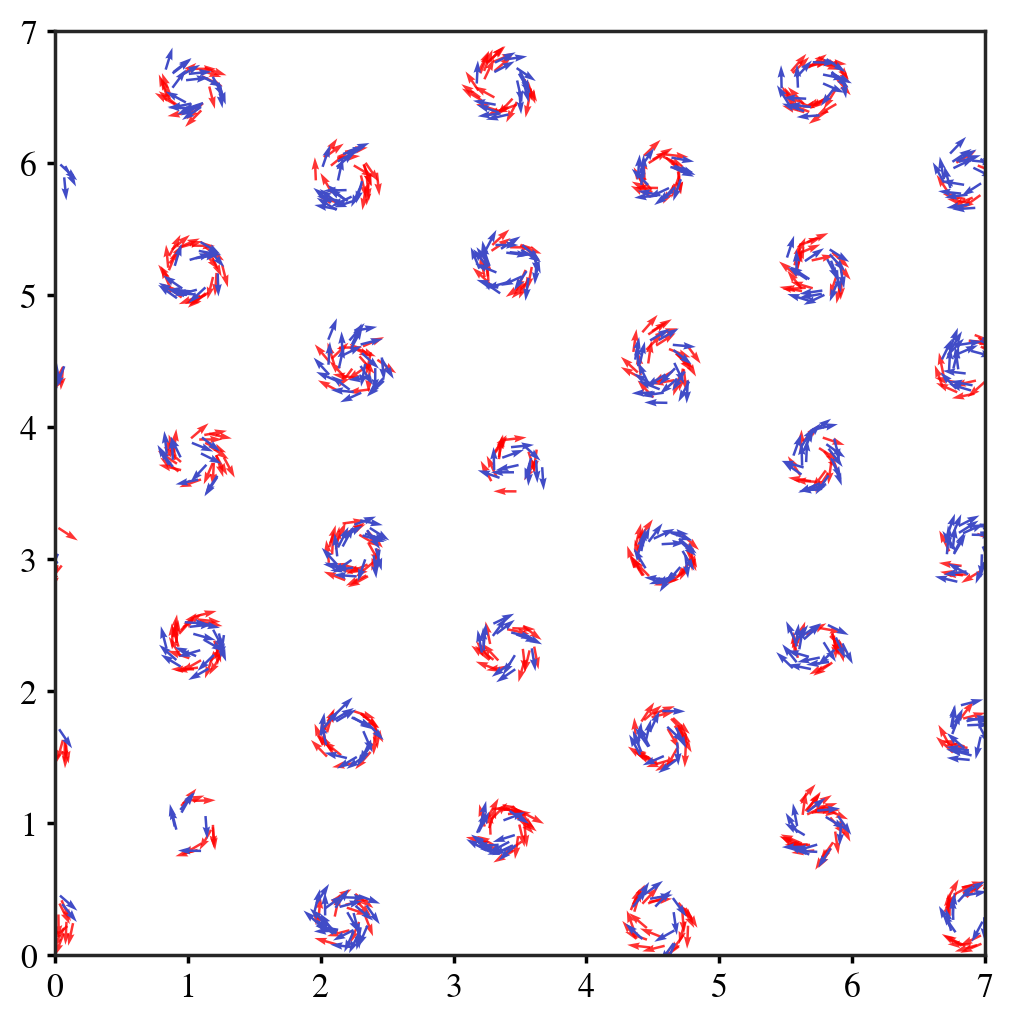
\includegraphics[width=0.35\textwidth]{./figs/snapshot.png}
    \caption{
        \label{fig:snapshot}
        Snapshot of the system at $t=80$ with $N=1000$, $K=19.2$, $\alpha =0.6\pi$, and $\omega _{\min}=0.1$, $\omega _{\max}=1$.
    }
\end{figure}

\bibliography{ref}

\end{document}